\section{Diseño (Desarrollo Teórico )}
\subsection{Diagrama a bloques del sistema}
En la siguiente figura, se muestra el diagrama a bloques del sistema, donde se destaca que es lo que
conforma cada una de las partes de potencia, microprocesador, comunicacion y perifericos.
    \begin{figure}[htp]
        \centering
            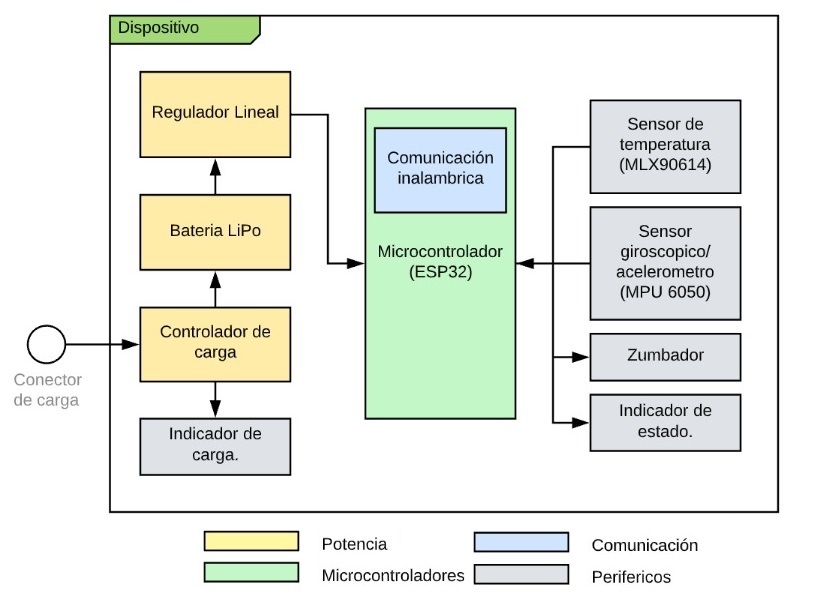
\includegraphics[width=\columnwidth]{system_block_diagram.png}
            \caption{Diagrama a bloques del sistema}
    \end{figure}
\subsection{Sensores}    
\textbf{MPU-9250}
    
    El MPU-9250 de InvenSense, es un dispositivo de medicion inercial (IMU) de 9 ejes, que combina un giroscopio de 3 ejes,
    un acelerómetro de 3 ejes, y un magnetómetro de 3 ejes, donde cada uno de estos cuenta con:
        \begin{itemize}
            \item Tres convertidores analógico-digitales (ADC) de 16 bits para digitalizar sus salidas. 
            \item Registros individuales de configuración, ya sea para rangos, frecuencia de muestreo, habilitación, etc.
        \end{itemize}

    La union de estos tres sensores y sus posibles configuraciones permiten el desarrollo de sistemas de deteccion/medicion de 
    movimientos con una buena fiabilidad. 

        \begin{figure}[htp]
            \centering
                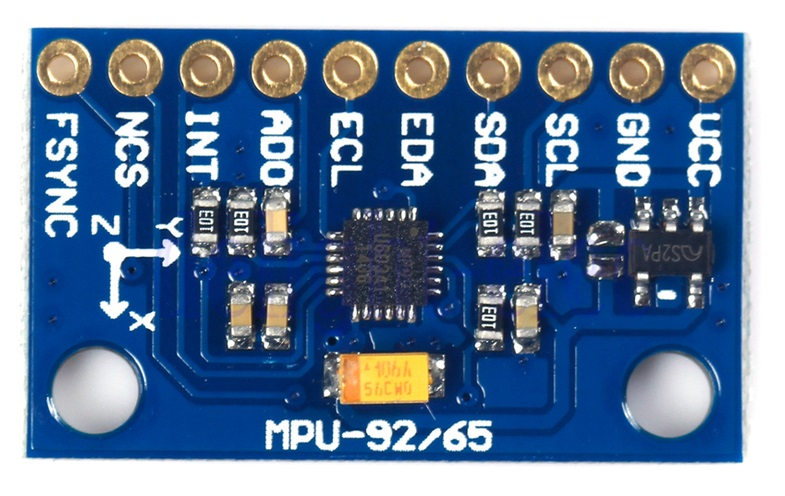
\includegraphics[width=5cm]{mpu_9250_board.png}
                \caption{MPU-9250 }
        \end{figure}

    \textbf{Caracteristicas}
        
    \begin{itemize}
        \item Giroscopio de tres ejes de salida digital con un rango de escala completa programable de $ \pm $250, $ \pm $500, $ \pm $1000 y $ \pm $2000°/seg.
        \item Acelerómetro de tres ejes de salida digital con un rango de escala completa programable de $ \pm $2g, $ \pm $4g, $ \pm $8g y $ \pm $16g.
        \item Sensor magnético monolítico de efecto Hall de 3 ejes con concentrador magnético con resolucion de 0,6T/LSB.
        \item Cuenta con interfaz para comunicacion por SPI y I2C.
    \end{itemize}
